\documentclass[11pt]{article}
\usepackage[letterpaper,margin=1in]{geometry}
\usepackage{amsmath,amssymb,amsfonts}
\usepackage{booktabs,tabularx,array,multirow}
\usepackage{graphicx,float,caption}
\usepackage{xcolor}
\usepackage{microtype}
\usepackage{enumitem}
\usepackage{cite}
\usepackage[hidelinks]{hyperref}
\usepackage{url}
\usepackage{xspace}

% Toggle this flag in the marked copy. The clean manuscript keeps revised
% passages black while the response-package copy renders them in red.
\newif\ifshowrevisions
\showrevisionstrue
\ifshowrevisions
  \newcommand{\revised}[1]{\textcolor{red}{#1}}
\else
  \newcommand{\revised}[1]{#1}
\fi

\definecolor{cbadred}{HTML}{C0392B}
\definecolor{modelblue}{HTML}{2874A6}
\definecolor{softgray}{HTML}{F3F5F7}
\newcommand{\method}{centered full-action DQN\xspace}
\newcommand{\R}{\mathbb{R}}
\DeclareMathOperator{\clip}{clip}

\title{\textbf{\revised{A Consistent DQN-Family Advantage in a Resource-Coupled Satellite-Ground Scheduling Benchmark}}}
\author{
Bocheng Yang$^{1}$, Lujie Zheng$^{1}$, Jian Liu$^{1,2,*}$, and Bo Chen$^{1,*}$\\[3pt]
\small $^{1}$School of Aerospace, Harbin Institute of Technology (Shenzhen), Shenzhen 518055, China\\
\small $^{2}$Guangxi Key Laboratory of Precision Navigation Technology and Application,\\[-2pt]
\small Guilin University of Electronic Technology, Guilin 541004, China\\
\small $^{*}$Correspondence: liujian2024@hit.edu.cn; hitchenbo@hit.edu.cn
}
\date{}

\begin{document}
\emergencystretch=2em
\maketitle
\input{generated/reviewer_macros.tex}
\color{red}% BEGIN STATE-COMPLETE REVISION
\input{generated/extended_macros.tex}
\color{black}% END STATE-COMPLETE REVISION

\begin{abstract}
\color{red}% BEGIN STATE-COMPLETE REVISION
Satellite-ground scheduling is a sequential control problem because each allocation changes resources available to later tasks. We investigate whether a deep Q-network (DQN) family captures this coupling more effectively than myopic, heuristic, contextual-bandit, and exact finite-horizon comparators. Six DQN objectives share an identical 24-dimensional state, architecture, replay, optimizer, interaction budget, \IndependentModelSeeds{} independently trained seeds, and held-out evaluation traces. The fully specified benchmark spans five coupled regimes and stresses compute, energy, thermal, and communication resources. Across all \DQNFamilyBelowMPCCount{} DQN objective--regime combinations, mean episode cost was below the corresponding strongest implemented non-DQN comparator, the four-step exact planner (MPC-4). In nominal conditions, DQN-family means were \DQNFamilyNominalMinCost--\DQNFamilyNominalMaxCost, compared with \MPCNominalCost{} for MPC-4 and 101.00 for the contextual bandit. Within-family differences were smaller and scenario dependent, showing that the main advance lies at the DQN-family rather than individual-objective level. Extending exact planning from one to six steps reduced cost but increased decision time from \PlannerTimeHOne{} to \PlannerTimeHSix{} ms. These results identify long-horizon value learning as an effective strategy for resource-coupled scheduling in this benchmark. Mission-derived utilities, hard constraints, and operational traces provide the next validation stage.
\color{black}% END STATE-COMPLETE REVISION
\end{abstract}

\color{red}% BEGIN STATE-COMPLETE REVISION
\noindent\textbf{Keywords:} deep Q-network variants; satellite edge computing; task scheduling; model-assisted reinforcement learning; full-action supervision.
\color{black}% END STATE-COMPLETE REVISION

\begin{figure}[!htbp]
\centering
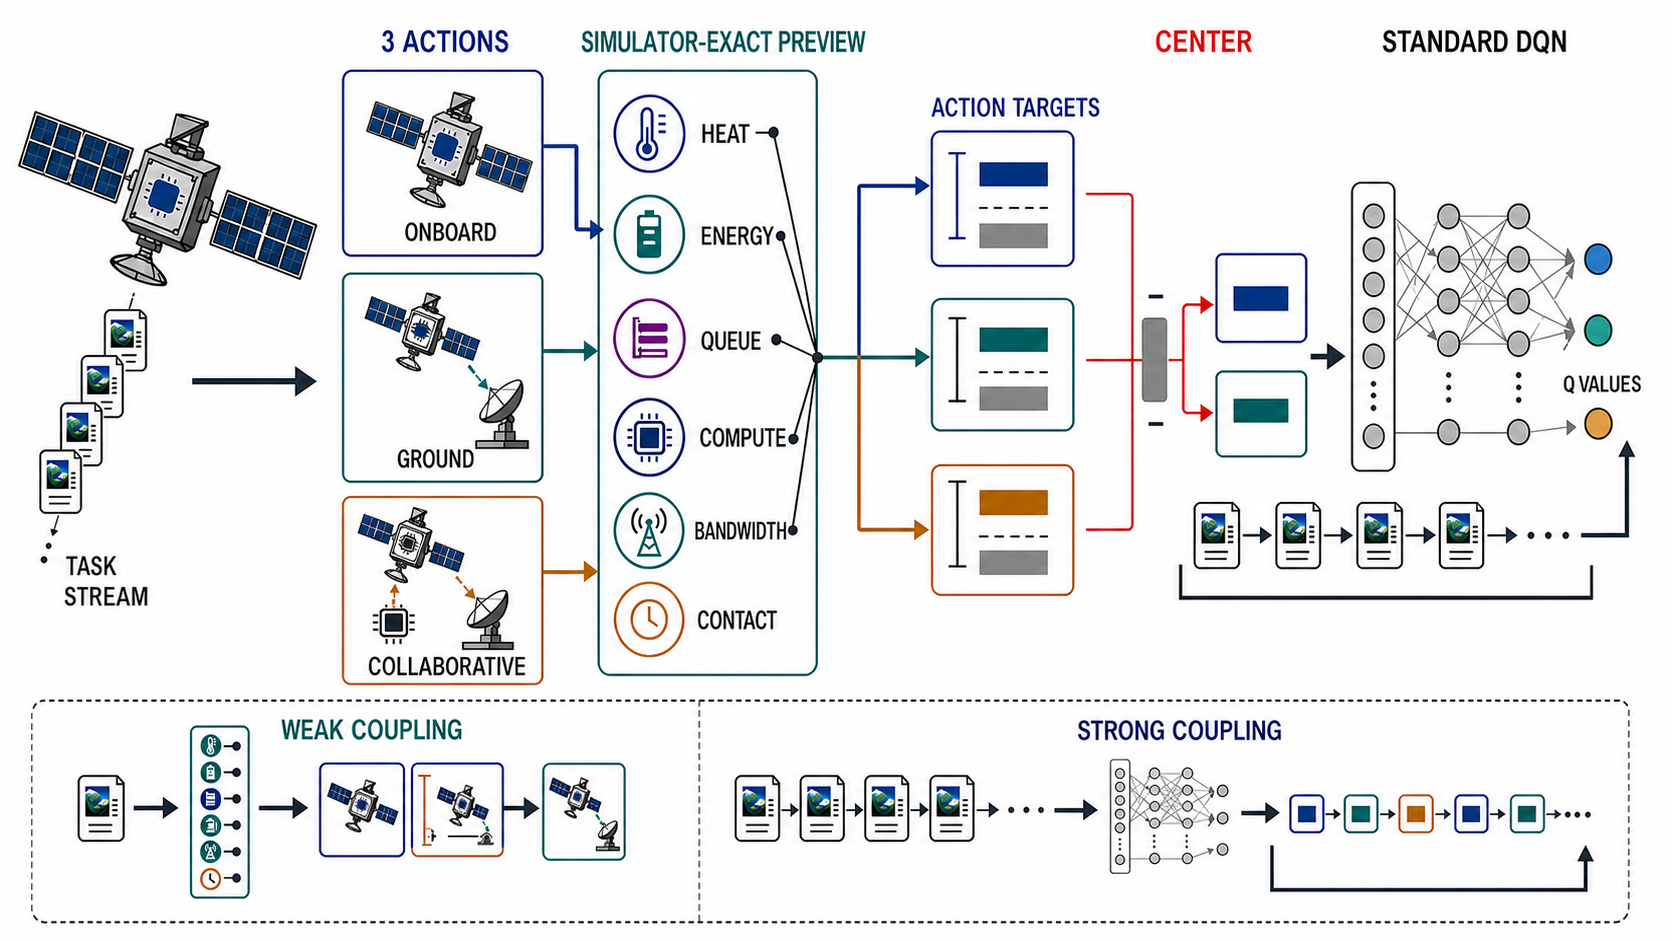
\includegraphics[width=0.98\textwidth,height=0.42\textheight,keepaspectratio]{figures/ai/fig_graphical_abstract_simulator_exact_arial.png}
\color{red}% BEGIN STATE-COMPLETE REVISION
\caption{Graphical overview of the centered full-action member of the evaluated DQN family. Simulator-exact analytical previews expose the immediate cost and six post-action resources for all three scheduling actions. Other family members remove centering, remove the bootstrap, use only factual transitions, or apply Double-DQN target evaluation. Preview information is restricted to training. The illustration is conceptual and encodes no quantitative results.}
\color{black}% END STATE-COMPLETE REVISION
\label{fig:graphical}
\end{figure}

\section{Introduction}

\color{red}% BEGIN STATE-COMPLETE REVISION
Earth-observation and communication satellites increasingly execute perception and decision workloads in orbit. Compact networks can reduce downlink demand and response latency under constrained onboard resources~\cite{9925218,10107454,10378728,10440355,10423050}. However, onboard execution consumes heat, energy, and compute capacity, whereas ground offloading consumes contact time and bandwidth. Effective scheduling must therefore coordinate onboard execution, complete offloading, and collaborative preprocessing over time.
\color{black}% END STATE-COMPLETE REVISION

\color{red}% BEGIN STATE-COMPLETE REVISION
Existing schedulers optimize constellation coordination, observation plans, service placement, deadlines, makespan, or energy use~\cite{RN8,RN10,RN20,RN22,RN23,RN27,RN28}. Here, every decision changes six resources that persist across task arrivals: heat, energy, queue occupancy, compute utilization, bandwidth, and remaining contact. An inexpensive action can therefore restrict the choices available for later tasks. This temporal coupling motivates a central question: can learned long-horizon values outperform transparent one-step and finite-horizon alternatives across changing resource conditions?
\color{black}% END STATE-COMPLETE REVISION

\color{red}% BEGIN STATE-COMPLETE REVISION
Standard DQN~\cite{mnih2015human,watkins1992q} learns one Bellman target from each factual tuple $(s_t,a_t,r_t,s_{t+1})$. In this setting, analytical resource equations can also evaluate every unexecuted action without advancing the environment or revealing later tasks. This structure enables a controlled test of both the DQN family and alternative ways to use full-action supervision during training.
\color{black}% END STATE-COMPLETE REVISION

\color{red}% BEGIN STATE-COMPLETE REVISION
We compare six DQN objectives: standard DQN, full-action Q, immediate advantage, centered full-action, Double DQN, and Double DQN with centered full-action supervision. A separate $\gamma=0$ contextual bandit provides a learned one-step comparator. Model-evaluated alternatives are available only during training; every deployed policy acts directly from its learned Q-values.
\color{black}% END STATE-COMPLETE REVISION

Our contributions are:

\begin{enumerate}[leftmargin=1.6em]
\color{red}% BEGIN STATE-COMPLETE REVISION
    \item We formulate resource-coupled satellite-ground scheduling as a reproducible 24-dimensional sequential benchmark with three processing modes and six persistent resources.
    \item We construct a controlled six-objective DQN family that varies factual supervision, full-action targets, centering, bootstrapping, and Double-DQN evaluation under matched training conditions.
    \item We establish a multilevel evaluation that separates the DQN-family result from smaller objective-specific effects using paired seed blocks, five stress regimes, and planning-depth analysis.
    \item We provide a scripted evidence chain linking simulator equations, transition audits, trained checkpoints, seed-level inference, generated tables, and publication figures.
\color{black}% END STATE-COMPLETE REVISION
\end{enumerate}

\color{red}% BEGIN STATE-COMPLETE REVISION
\section{Related Work and Study Positioning}
\color{black}% END STATE-COMPLETE REVISION

\subsection{Satellite-ground scheduling}

\color{red}% BEGIN STATE-COMPLETE REVISION
Satellite schedulers cover constellation coordination, observation planning, service placement, and energy-aware offloading~\cite{RN8,RN10,RN20,RN22,RN23,RN27,RN28}. Our setting combines an explicit cost for every action with resource carryover between task arrivals. The one-step objective is therefore observed rather than hidden. The benchmark asks whether a learned value function can exploit consequences that persist beyond this observed one-step cost.
\color{black}% END STATE-COMPLETE REVISION

\color{red}% BEGIN STATE-COMPLETE REVISION
\subsection{Model use and full-action learning}
\color{black}% END STATE-COMPLETE REVISION

\color{red}% BEGIN STATE-COMPLETE REVISION
Dyna established predicted experience for value learning and planning~\cite{sutton1991dyna}, and fitted dynamics can accelerate deep Q-learning~\cite{gu2016continuous}. Counterfactual data fusion and causal augmentation construct transitions under structural assumptions~\cite{forney2017counterfactual,armengol2024caiac}. Counterfactual credit assignment instead separates action influence from future randomness~\cite{mesnard2021counterfactual}. Recent work also studies multi-action generative interfaces and joint quantities across action outcomes~\cite{kaya2026joint}. Together, these studies establish several routes for incorporating modeled alternatives into reinforcement learning.
\color{black}% END STATE-COMPLETE REVISION

\color{red}% BEGIN STATE-COMPLETE REVISION
Advantage learning widens action gaps through modified operators~\cite{bellemare2016gap}. The centered full-action DQN objective instead retains the selected Bellman operator and adds supervised within-state action gaps. Table~\ref{tab:closest_methods} distinguishes this construction from related mechanisms. Joint MDPs provide the closest multi-action interface~\cite{kaya2026joint}, while full-action Q provides the closest empirical control. Our contribution is a controlled family-level evaluation that separates shared DQN performance from the smaller effects of target construction, centering, and bootstrapping.

In this manuscript, ``counterfactual'' denotes a model-evaluated one-step outcome for an unexecuted action under the same current task and exogenous state. It does not denote an identified causal effect from observational data.

\begin{table}[H]
\centering
\caption{Feature comparison with the closest method families. ``All actions'' means that one learning update can use modeled outcomes for every discrete action at the sampled state.}
\label{tab:closest_methods}
\small
\begin{tabularx}{\textwidth}{lXXX}
\toprule
Method family & Source of modeled information & How it enters learning & Relation to this study \\
\midrule
Dyna and local model-based acceleration~\cite{sutton1991dyna,gu2016continuous} & Learned or fitted dynamics & Simulated experience or local rollouts & Does not use one simultaneous analytical label per action in the reported auxiliary loss \\
Causal counterfactual augmentation~\cite{armengol2024caiac} & Structural assumptions and offline trajectories & Synthetic transitions augment the training distribution & Targets distributional coverage rather than within-state Bellman action gaps \\
Counterfactual credit assignment~\cite{mesnard2021counterfactual} & Future-conditioned trajectory information & Policy-gradient baseline or critic & Model-free and trajectory-conditioned rather than analytical one-step action enumeration \\
Joint MDPs~\cite{kaya2026joint} & Multi-action sample transition model & Joint action-outcome quantities and Bellman operators & Closest formal interface; it does not specify the centered DQN auxiliary loss evaluated here \\
This study & Deterministic analytical one-step transition for three actions & Auxiliary full-action Bellman targets; no replay insertion & Same real interactions as DQN, but three modeled action outcomes per eligible training state \\
\bottomrule
\end{tabularx}
\end{table}
\color{black}% END STATE-COMPLETE REVISION

\section{System Model and Immediate-Cost Quantification}
\label{sec:system}

At task arrival $t$, a satellite selects one of three actions:
\begin{equation}
\mathcal A=\{\alpha_s,\alpha_g,\alpha_{s\&g}\},
\end{equation}
where $\alpha_s$ executes onboard and downlinks the result, $\alpha_g$ downlinks the complete input for ground execution, and $\alpha_{s\&g}$ performs onboard preprocessing followed by ground execution.

\begin{figure}[H]
\centering
\includegraphics[width=0.98\textwidth,height=0.42\textheight,keepaspectratio]{figures/ai/fig_system_modes_arial.png}
\caption{Three satellite-ground processing pathways. Each arriving task is executed onboard, transferred for ground execution, or preprocessed collaboratively before ground completion. The analytical transition model returns the immediate cost and the post-action heat, energy, queue occupancy, compute utilization, bandwidth, and remaining contact.}
\label{fig:system}
\end{figure}

\subsection{Implemented immediate-cost model}

\color{red}% BEGIN STATE-COMPLETE REVISION
The experiments use the dimensionless linear cost implemented by the internally consistent synthetic simulator. Let $x_k$ denote the 15 task descriptors in Table~\ref{tab:state_dictionary}. Each descriptor is normalized as
\color{black}% END STATE-COMPLETE REVISION
\begin{equation}
\bar x_k=\clip(x_k/s_k,0,1.5),
\end{equation}
where $s_k$ is the corresponding scale. For inherited normalized bandwidth $b$, the available return rate is $R(b)=2.2+217.8b$ Mbit s$^{-1}$. The three action latencies are
\begin{align}
L_s&=x_3+1000x_6/R(b),\notag\\
L_g&=x_8+1000x_9/R(b),\notag\\
L_{s\&g}&=1000x_{12}/4+x_{13}+1000x_{15}/R(b).
\label{eq:latencies}
\end{align}
The implemented immediate costs are
\begin{align}
c_s^{imm}={}&0.70\bar x_1+0.65\bar x_2+0.00045L_s+0.55\bar x_5
+0.35\bar x_6+0.35h+0.12(1-e),\notag\\
c_g^{imm}={}&0.45\bar x_7+0.00045L_g+0.55\bar x_9
+0.35(0.28-\tau)_+,\notag\\
c_{s\&g}^{imm}={}&0.55(\bar x_{10}+\bar x_{11})+0.55\bar x_{14}
+0.00045L_{s\&g}+0.45\bar x_{15}\notag\\
&+0.18h+0.12q+0.18(0.22-\tau)_+.
\label{eq:implemented_costs}
\end{align}
Here $h$, $e$, $q$, and $\tau$ are inherited heat, remaining energy, queue occupancy, and contact duration. The weights are fixed simulator assumptions rather than fitted mission utilities. They are applied identically during training, counterfactual preview, MPC evaluation, and deployment evaluation. Automated tests reproduce Eq.~\eqref{eq:implemented_costs} from the 15 raw descriptors and compare it with all three code outputs.

\begin{table}[H]
\centering
\color{red}% BEGIN STATE-COMPLETE REVISION
\caption{Implemented 15-dimensional task descriptor dictionary. The complete 24-dimensional observation appends normalized time, sine and cosine of link phase, and six resource coordinates: $h$, $e$, $q$, compute utilization $u$, bandwidth $b$, and contact duration $\tau$.}
\color{black}% END STATE-COMPLETE REVISION
\label{tab:state_dictionary}
\resizebox{\textwidth}{!}{\input{generated/table_state_dictionary.tex}}
\end{table}

\color{red}% BEGIN STATE-COMPLETE REVISION
\subsection{Internally consistent task and communication generator}
\color{black}% END STATE-COMPLETE REVISION

\color{red}% BEGIN STATE-COMPLETE REVISION
The simulator does not sample heat, workload, data volume, and latency independently. It first draws correlated latent variables $(v_t,w_t)$ with correlation parameter 0.68 and maps them through a logistic transform to raw data volume $D_t\in[8,64]$ Mbit and workload $W_t\in[0.25,4.0]$ GFLOP. Result and collaborative-feature volumes are
\color{black}% END STATE-COMPLETE REVISION
\begin{equation}
D_t^{res}=r_tD_t,\quad r_t\in[0.01,0.05],\qquad
D_t^{feat}=f_tD_t,\quad f_t\in[0.08,0.30].
\end{equation}
The implementation enforces $D_t^{res}\le D_t^{feat}\le D_t$. A workload-dependent fraction $p_t\in[0.20,0.45]$ is processed onboard in the collaborative mode. Given onboard and ground rates $R_s=4$ and $R_g=80$ GFLOP s$^{-1}$, processing time is derived as $W/R$, rather than sampled separately. Compute power rises monotonically from 4 to 20 W with workload; compute heat is 0.78 times compute energy. Transmission time is data volume divided by the effective return rate
\begin{equation}
R_t^{link}=2.2+217.8b_t\quad\text{Mbit s}^{-1},
\end{equation}
and transmission heat is 0.55 times transmit energy. These values are engineering envelopes, not fitted flight distributions. Their scale is consistent with the range of modern SmallSat computing-system power reported by NASA and with NASA ground-network examples spanning 2.2 Mbit s$^{-1}$ S-band to 220 Mbit s$^{-1}$ X-band returns~\cite{nasa2026avionics,nasa2026ground}. The bounded data-reduction factors represent the bandwidth-reduction role of onboard image compression, not a claim about one instrument-specific codec~\cite{ccsds122}. Table~\ref{tab:parameters} states every implemented assumption.

\begin{table}[H]
\centering
\color{red}% BEGIN STATE-COMPLETE REVISION
\caption{Modeled engineering primitives and provenance of the current simulator. Values define a transparent synthetic envelope; they are not presented as a fitted flight distribution.}
\color{black}% END STATE-COMPLETE REVISION
\label{tab:parameters}
\resizebox{\textwidth}{!}{\input{generated/table_parameter_provenance.tex}}
\end{table}

An automated audit generated \PhysicalAuditTasks{} tasks before training. All values were finite and positive, all data-flow inequalities held, and the empirical raw-data--workload correlation was \PhysicalCorrDataWork. Figure~\ref{fig:physical} shows the resulting dependence structure. Constant-rate columns have zero variance and are therefore excluded from correlation coefficients.

\begin{figure}[H]
\centering
\includegraphics[width=0.98\textwidth]{figures/fig_physical_generator.pdf}
\color{red}% BEGIN STATE-COMPLETE REVISION
\caption{Internal-consistency audit of the synthetic generator. (a) A legibility sample of 2,000 of 20,000 tasks; color encodes heat derived from compute energy. (b) Correlations computed from all 20,000 tasks. No fitted flight distribution is implied.}
\color{black}% END STATE-COMPLETE REVISION
\label{fig:physical}
\end{figure}

\subsection{Complete stochastic generator and action-load specification}
\label{sec:complete_simulator}

For independent reconstruction, this subsection states the remaining simulator functions that enter the transition. Let $u_D,\epsilon_W\sim\mathcal N(0,1)$ independently, $u_W=0.68u_D+\sqrt{1-0.68^2}\epsilon_W$, and $g(u)=[1+\exp(-1.55u)]^{-1}$. Nominal raw volume and workload are
\begin{equation}
D=8+56g(u_D)\ {\rm Mbit},\qquad W=0.25+3.75g(u_W)\ {\rm GFLOP}.
\label{eq:primitive_generator}
\end{equation}
The burst interval occupies indices $\lfloor T/3\rfloor$ through $\lfloor T/3\rfloor+\max(4,\lfloor T/4\rfloor)-1$ and multiplies both quantities by 1.45. With independent $U_r,U_f\sim\mathcal U(0,1)$,
\begin{align}
r&=0.01+0.04U_r,\qquad f=0.08+0.22\clip[0.65g(u_W)+0.35U_f,0,1],\notag\\
\color{red}% BEGIN STATE-COMPLETE REVISION
p&=0.20+0.25g(u_W),\qquad D^{res}=rD,\quad D^{feat}=fD,\quad W^{pre}=pW,\notag\\
n&=\operatorname{round}\{6+43\clip[0.60g(u_W)+0.40g(u_D),0,1]\},\qquad x_5=n^2.
\color{black}% END STATE-COMPLETE REVISION
\label{eq:primitive_ratios}
\end{align}
Onboard and ground rates are 4 and 80~GFLOP~s$^{-1}$, respectively. Compute power is $P_c=4+16\clip(W/4.8,0,1)^{0.70}$~W, and transmit power is 6~W. Compute and transmit heat are 0.78 and 0.55 times their corresponding energy use. These definitions generate all 15 coordinates in Table~\ref{tab:state_dictionary}.

At reset, a single phase $\phi\sim\mathcal U(0,2\pi)$ generates the exogenous link trace
\begin{align}
\bar b_t&=\clip\left\{\kappa_b[0.62+0.23\sin(2\pi t/24+\phi)+\epsilon^b_t]-I_{link},0.12,1\right\},\notag\\
\bar\tau_t&=\clip\left\{0.55+0.35\sin(2\pi t/31+\phi/2)+\epsilon^\tau_t,0.08,1\right\},
\label{eq:link_trace}
\end{align}
where $\epsilon^b_t\sim\mathcal N(0,0.06^2)$, $\epsilon^\tau_t\sim\mathcal N(0,0.04^2)$, $\kappa_b$ is the sensitivity multiplier, and $I_{link}=0.22$ only in the link-limited regime. All episode tasks and link states are drawn at reset from one seeded NumPy generator.

The normalized action loads used in Eq.~\eqref{eq:transition} are stated here in action order $(\alpha_s,\alpha_g,\alpha_{s\&g})$:
\begin{align}
\widehat w&=(W,0.05W,W)/4.8,\qquad
\widehat Q=(x_1,0.20x_7,x_{10}+x_{11})/100,\notag\\
\widehat B&=(x_6,x_9,x_{15})/76.8,\notag\\
\Delta e&=\kappa_e\left(0.012+0.042\widehat w_1,
0.007+0.025\widehat B_2/b,
0.010+0.025\widehat w_3+0.018\widehat B_3/b\right),\notag\\
\Delta q&=\left(0.055\widehat w_1(1+u),
0.048\widehat B_2/b,
0.030(\widehat w_3+\widehat B_3/b)\right),\notag\\
\mu&=\left(0.030(1-u),0.035b\tau,0.032(1-0.5u)\right),\notag\\
\ell&=(0.02,0.18\widehat B_2,0.12\widehat B_3).
\label{eq:action_loads}
\end{align}
\color{red}% BEGIN STATE-COMPLETE REVISION
Here divisions by $b$ use $\max(b,0.1)$. The utilization targets in Eq.~\eqref{eq:transition} are $(\widehat w_1,0.10\widehat B_2,0.55\widehat w_3)$. Initial resources are $(h,e,q,u)=(0.22,0.88,0.12,0.18)$ except that energy-limited episodes use $e=0.62$ and thermal-stress episodes use $h=0.42$. Each episode terminates after exactly 64 executed actions; the terminal Bellman multiplier is zero. Energy and other resources remain soft-constrained clipped accounting states. In particular, $e=0$ does not represent a conserved battery state because it neither masks infeasible actions nor terminates an episode, and clipping does not retain the magnitude of an energy deficit.
\color{black}% END STATE-COMPLETE REVISION

\section{Sequential Scheduling Formulation}
\label{sec:mdp}

\subsection{State and transition}

\color{red}% BEGIN STATE-COMPLETE REVISION
The normalized 24-dimensional state is
\color{black}% END STATE-COMPLETE REVISION
\begin{equation}
\color{red}% BEGIN STATE-COMPLETE REVISION
s_t=[x_t,\eta_t,z_t],\qquad
\eta_t=[t/(T-1),\sin\phi,\cos\phi],\qquad
z_t=[h_t,e_t,q_t,u_t,b_t,\tau_t],
\color{black}% END STATE-COMPLETE REVISION
\end{equation}
\color{red}% BEGIN STATE-COMPLETE REVISION
where $x_t\in\R^{15}$ contains the task inputs defined in Table~\ref{tab:state_dictionary}. The context vector $\eta_t$ exposes absolute episode time and the reset-level link phase that determine the time-varying task and link distributions. The remaining task and link innovations are independent draws conditional on this context. The six resource variables denote normalized heat, remaining energy, queue occupancy, compute utilization, bandwidth, and contact duration. Thus, within each fixed regime, the transition distribution is conditioned on all persistent simulator variables rather than on a hidden reset phase.
\color{black}% END STATE-COMPLETE REVISION

Executing action $a_t$ changes resources before the next exogenous task arrives. The implemented transition is
\begin{align}
h_{t+1}&=\clip(0.86h_t+0.17c\widehat Q_t^{(a_t)},0,1.3),\notag\\
e_{t+1}&=\clip(e_t+0.006-c\Delta e_t^{(a_t)},0,1),\notag\\
q_{t+1}&=\clip(q_t+c(\Delta q_t^{(a_t)}-\mu_t^{(a_t)}),0,1.3),\notag\\
u_{t+1}&=\clip(0.68u_t+0.32c\widehat w_t^{(a_t)},0,1.2),\notag\\
b_{t+1}&=\clip(\bar b_{t+1}-c\ell_t^{(a_t)},0.08,1),\notag\\
\tau_{t+1}&=\clip(\bar\tau_{t+1}-0.10c\widehat B_t^{(a_t)},0.05,1).
\label{eq:transition}
\end{align}
Here $\widehat Q$, $\widehat w$, and $\widehat B$ are normalized action-specific heat, work, and data demands. The terms $\Delta e$, $\Delta q$, $\mu$, and $\ell$ are the deterministic resource-use, queue, service, and link-occupation functions defined in Eq.~\eqref{eq:action_loads}. Exogenous link variables $\bar b$ and $\bar\tau$ follow Eq.~\eqref{eq:link_trace} and are sampled before each episode. Coupling $c=0$ removes action-dependent carryover, $c=0.5$ weakens it, and $c=1$ defines full coupling.

\subsection{Reward and standard DQN backbone}

The reward is the negative immediate cost plus post-decision feasibility penalties:
\begin{align}
r_t={}&-c_t^{imm}-c\big[12(h_{t+1}-0.78)_+ +15(0.18-e_{t+1})_+\notag\\
&+8(q_{t+1}-0.75)_+ +10\mathbf 1_{a_t\ne\alpha_s}(0.14-\tau_t)_+\big].
\label{eq:reward}
\end{align}
The DQN uses the unmodified factual target
\begin{equation}
y_t=r_t+\gamma(1-d_t)\max_{a'}Q_{\bar\theta}(s_{t+1},a'),
\label{eq:factual}
\end{equation}
and factual loss
\begin{equation}
L_{DQN}=\mathcal H\big(Q_\theta(s_t,a_t),y_t\big),
\end{equation}
where $\mathcal H$ denotes the Huber loss. The target network both selects and evaluates the maximizing action, as required by standard DQN.

\color{red}% BEGIN STATE-COMPLETE REVISION
\section{DQN Variants with Model-Evaluated Full-Action Targets}
\color{black}% END STATE-COMPLETE REVISION
\label{sec:method}

\color{red}% BEGIN STATE-COMPLETE REVISION
The DQN family shares the factual target and loss in Eq.~\eqref{eq:factual}. Its model-assisted variants add a training-only auxiliary path that can supply labels for unexecuted actions. The following construction defines the centered full-action member; the experimental design then removes centering, removes the bootstrap, or changes target evaluation to identify how these choices alter performance.
\color{black}% END STATE-COMPLETE REVISION

\subsection{Side-effect-free full-action preview}

For every replayed factual state, the analytical transition evaluates each $a\in\mathcal A$:
\begin{equation}
(\tilde \ell_{t,a},\tilde z'_{t,a})=F_{preview}(x_t,z_t,a).
\end{equation}
Here $\tilde \ell_{t,a}$ contains the immediate cost and post-decision feasibility penalty for action $a$. The preview does not advance time, mutate state, alter trajectories, or consume random numbers. Before action selection it computes only the current-task cost and six post-action resources. The factual action is then executed once, after which the next exogenous task $x_{t+1}$ is revealed and the replay tuple is completed. During a later replay update, all alternatives reuse this observed next task and exogenous link trace. The counterfactual next state therefore replaces only the six endogenous resource coordinates:
\begin{equation}
\color{red}% BEGIN STATE-COMPLETE REVISION
\tilde s'_{t,a}=[x_{t+1},\eta_{t+1},\tilde z'_{t,a}].
\color{black}% END STATE-COMPLETE REVISION
\end{equation}
Evaluation and deployment never call the preview interface.

\subsection{All-action counterfactual Bellman targets}

The simulator-exact one-step outcome yields
\begin{equation}
\tilde y_{t,a}=-\tilde \ell_{t,a}+\gamma(1-d_t)
\max_{a'}Q_{\bar\theta}(\tilde s'_{t,a},a').
\label{eq:cf_target}
\end{equation}
The targets create no multi-step rollout and insert no counterfactual transition into replay. They are used only after state-wise centering in the complete method below.

\subsection{Centered advantage distillation}

Absolute targets in Eq.~\eqref{eq:cf_target} share a bootstrapped state-value offset. Deployment selects $\arg\max_a Q(s,a)$, so a common additive offset cannot change the action. We define predicted and target centered advantages as
\begin{align}
\widehat A_{t,a}&=Q_\theta(s_t,a)-\frac{1}{|\mathcal A|}\sum_jQ_\theta(s_t,j),\notag\\
\tilde A_{t,a}&=\tilde y_{t,a}-\frac{1}{|\mathcal A|}\sum_j\tilde y_{t,j}.
\label{eq:center}
\end{align}
The advantage and total losses are
\begin{align}
L_{adv}&=\frac{1}{|\mathcal A|}
\sum_{a\in\mathcal A}\mathcal H(\widehat A_{t,a},\tilde A_{t,a}),\notag\\
\color{red}% BEGIN STATE-COMPLETE REVISION
L_{CFA}&=L_{DQN}+\lambda L_{adv}.
\color{black}% END STATE-COMPLETE REVISION
\label{eq:cbad}
\end{align}
The factual term anchors the absolute Q scale, while $L_{adv}$ teaches all action gaps. The only added algorithmic hyperparameter is $\lambda$.

\begin{figure}[H]
\centering
\includegraphics[width=0.98\textwidth,height=0.43\textheight,keepaspectratio]{figures/ai/fig_cbad_mechanism_simulator_exact_arial.png}
\color{red}% BEGIN STATE-COMPLETE REVISION
\caption{Training-only centered full-action mechanism. The upper path retains the factual standard-DQN target and Huber loss. The lower path previews all three actions, constructs three Bellman targets, centers them within state, and distills their relative advantages. Both losses update the online Q-network; the target network is synchronized only at the shared fixed interval. Preview outputs are unavailable during evaluation and deployment.}
\color{black}% END STATE-COMPLETE REVISION
\label{fig:mechanism}
\end{figure}

\begin{figure}[H]
\centering
\fbox{\begin{minipage}{0.93\textwidth}
\color{red}% BEGIN STATE-COMPLETE REVISION
\textbf{Algorithm 1: DQN training with centered full-action supervision}
\color{black}% END STATE-COMPLETE REVISION
\begin{enumerate}[leftmargin=1.6em,itemsep=2pt,topsep=4pt]
\item Initialize uniform replay $\mathcal D$, online $Q_\theta$, and target $Q_{\bar\theta}\leftarrow Q_\theta$.
\item At each real step, observe $s_t$ and preview current-task outcomes $(\tilde \ell_{t,a},\tilde z'_{t,a})$ for all actions without side effects.
\item Select $a_t$ by the shared epsilon-greedy schedule and execute it once. After $x_{t+1}$ is revealed, store the factual tuple plus the previously computed previews.
\item When an update is due, sample one uniform mini-batch, compute the factual loss, compute Eqs.~\eqref{eq:cf_target} and \eqref{eq:center}, and update $\theta$ using Eq.~\eqref{eq:cbad}.
\item Synchronize $Q_{\bar\theta}$ at the shared fixed interval.
\end{enumerate}
\end{minipage}}
\par\smallskip
\caption*{Training previews are never used for evaluation or deployment.}
\label{alg:cbad}
\end{figure}

\section{Experimental Design and Settings}
\label{sec:experiments}

\subsection{Design principles}

\color{red}% BEGIN STATE-COMPLETE REVISION
The design addresses four comparisons. Standard DQN versus its centered full-action variant measures the effect of adding the complete auxiliary objective to an unchanged factual DQN backbone. Uncentered full-action Q and centered immediate-cost targets receive the same three modeled outcomes per state. They match the type and count of model outputs. They do not by themselves isolate centering or Bellman bootstrapping because their target scales differ and their auxiliary weights were not tuned separately. Double DQN with and without centered full-action supervision assesses whether the fixed auxiliary implementation has a similar descriptive effect when action selection and target evaluation are decoupled~\cite{vanhasselt2016double}. The $c\in\{0,0.5,1\}$ regimes and planners with $H\in\{1,2,4,6\}$ bound the family comparison as the implemented objective and planning depth change.
\color{black}% END STATE-COMPLETE REVISION

\color{red}% BEGIN STATE-COMPLETE REVISION
Standard DQN and its centered full-action variant share every component except the auxiliary objective. They use the same input, network, replay, exploration, optimizer, update cadence, target synchronization, and gradient clipping. The full-action Q control applies the same auxiliary weight directly to the three uncentered Bellman targets. The immediate-advantage control centers the negative analytical one-step costs but omits their bootstrapped future values. Both Double-DQN variants use online-network action selection with target-network evaluation in factual and auxiliary Bellman targets. Dueling networks, prioritized replay, multi-step returns, noisy networks, and distributional value learning remain outside the comparison.
\color{black}% END STATE-COMPLETE REVISION

\color{red}% BEGIN STATE-COMPLETE REVISION
The auxiliary weight was fixed before the internally consistent simulator experiment. A preceding calibration with model seeds 700--703 compared $\lambda\in\{0.1,0.3,1,3\}$. It selected $\lambda=0.3$ by maximizing the worst relative improvement of the centered full-action variant across five coupled regimes, with the smaller weight as the tie-break. This selection rule was specific to the centered objective. The uncentered full-action, immediate-advantage, and Double-DQN auxiliary variants inherited $\lambda=0.3$ without method-specific calibration. Because auxiliary losses differ in scale and error structure, their comparisons are fixed-coefficient implementation comparisons rather than a factorial identification of centering or bootstrapping. The calibration used an earlier simulator version and is a prior specification rather than evidence from the current generator. Confirmation and all component comparisons use seeds 800--819 without post hoc removal, replacement, or selection. Every learned policy was trained only on the nominal $c=1$ distribution.
\color{black}% END STATE-COMPLETE REVISION

\begin{figure}[!htbp]
\centering
\includegraphics[width=0.98\textwidth,height=0.42\textheight,keepaspectratio]{figures/ai/fig_experiment_protocol_20seeds_arial.png}
\color{red}% BEGIN STATE-COMPLETE REVISION
\caption{Prespecification and confirmation protocol. An earlier-simulator calibration with four seeds selected $\lambda=0.3$ for the centered full-action objective before the current synthetic experiment. Other auxiliary objectives inherited this coefficient without method-specific tuning. Twenty disjoint confirmation seeds, 800--819, are each evaluated on 20 shared held-out traces in seven regimes, with no current-generator tuning or seed exclusion.}
\color{black}% END STATE-COMPLETE REVISION
\label{fig:protocol}
\end{figure}

\subsection{Training configuration}

\color{red}% BEGIN STATE-COMPLETE REVISION
Each network has 24 inputs, hidden widths 128--128--64, ReLU activations, and three outputs. Every model receives 600 episodes of 64 tasks, totaling 38,400 real interactions. Fixed settings are $\gamma=0.97$, learning rate $3\times10^{-4}$, batch size 128, replay capacity 100,000, and gradient-norm limit 10. Training begins after 128 transitions and performs one update every four interactions. The checkpoint field \texttt{target\_interval=250} is evaluated only on update calls; because updates occur at interaction counts divisible by four, synchronization occurs every 500 real interactions, equivalent to 125 optimizer updates. Epsilon decreases linearly from 1 to 0.05 over 13,440 interactions.
\color{black}% END STATE-COMPLETE REVISION

\color{red}% BEGIN STATE-COMPLETE REVISION
The contextual bandit uses the same network, optimizer, exploration schedule, and interaction budget, with $\gamma=0$. It therefore learns the modeled one-step reward without a long-horizon Bellman term. Uniform replay stores only one-step factual transitions, with preview outputs attached as auxiliary training data. Standard DQN and Double DQN use no analytical alternative-action labels. The four auxiliary variants evaluate three modeled outcomes at every real interaction. The checkpoint manifest records these counts, optimizer updates, and wall time for every trained model.
\color{black}% END STATE-COMPLETE REVISION

\color{red}% BEGIN STATE-COMPLETE REVISION
All reported experiments use the internally consistent synthetic generator described above. Link bandwidth and contact follow bounded noisy periodic traces generated at reset. Burst and thermal-stress episodes multiply raw data and workload by 1.45 during one contiguous interval; all dependent heat, energy, latency, and transmission quantities are recomputed from those primitives. An earlier independently sampled generator is retained only as a historical reproducibility mode and is not used for the reported results.
\color{black}% END STATE-COMPLETE REVISION

\subsection{Seven evaluation regimes}

\color{red}% BEGIN STATE-COMPLETE REVISION
The seven regimes include two composite coupling-boundary conditions and five fully coupled operating conditions:
\color{black}% END STATE-COMPLETE REVISION

\begin{enumerate}[leftmargin=1.6em]
\color{red}% BEGIN STATE-COMPLETE REVISION
    \item \textbf{Static ($c=0$):} removes action-dependent state transitions and scales delayed feasibility penalties to zero.
    \item \textbf{Reduced coupling ($c=0.5$):} halves action-dependent resource effects and the delayed feasibility-penalty scale.
\color{black}% END STATE-COMPLETE REVISION
    \item \textbf{Nominal ($c=1$):} matches the fully coupled training distribution.
    \item \textbf{Burst:} increases contiguous compute and thermal demand.
    \item \textbf{Link-limited:} reduces the available bandwidth trace by 0.22 before clipping.
    \item \textbf{Energy-limited:} lowers initial energy from 0.88 to 0.62.
    \item \textbf{Thermal-stress:} raises initial heat from 0.22 to 0.42 and includes the burst interval.
\end{enumerate}

\color{red}% BEGIN STATE-COMPLETE REVISION
The first two regimes are composite interventions because the same $c$ appears in both the transition in Eq.~\eqref{eq:transition} and the delayed-penalty term in Eq.~\eqref{eq:reward}. They therefore do not isolate action-dependent carryover from reward rescaling. The remaining five regimes retain $c=1$. Models trained at $c=1$ are transferred to the two boundary conditions without retraining. These rows measure behavior under a joint objective-and-dynamics shift rather than the best policy attainable at lower coupling.
\color{black}% END STATE-COMPLETE REVISION

\subsection{Planning comparator, outcomes, and inference}

\color{red}% BEGIN STATE-COMPLETE REVISION
The deployment comparison includes immediate-cost argmin, a contextual bandit, a prespecified resource-threshold heuristic, standard DQN, \method, and exhaustive finite-horizon model-based planning. The threshold rule selects ground processing when $h>0.72$ or $e<0.24$ and both $b>0.28$ and $\tau>0.18$; under the same heat or energy condition it otherwise selects collaborative processing. If that condition is absent, it selects onboard processing when $b<0.22$ or $\tau<0.14$, collaborative processing when $q>0.70$, and immediate-cost argmin otherwise. These thresholds were hand specified and not fitted to the evaluation traces. Fixed onboard and fixed ground policies always select $\alpha_s$ and $\alpha_g$, respectively. At every real decision, the planner enumerates all $3^H$ action sequences over the next $H$ known tasks and link states, minimizes discounted modeled cost with $\gamma=0.97$, executes only the first action, and replans. The primary table retains $H=4$. A separate nominal analysis evaluates $H\in\{1,2,4,6\}$ on 400 unique held-out traces and reports wall-clock cost per decision. Each planner is exact only for its stated perfect-forecast objective, not for the 64-step global problem.
\color{black}% END STATE-COMPLETE REVISION

\color{red}% BEGIN STATE-COMPLETE REVISION
The primary outcome is the undiscounted episode total cost
\begin{equation}
C_{\mathrm{episode}}=\sum_{t=0}^{T-1}\left(c^{\mathrm{imm}}_t+p_t\right)=-\sum_{t=0}^{T-1}r_t,
\label{eq:episode_cost}
\end{equation}
where $p_t$ is the complete nonnegative penalty inside the square brackets in Eq.~\eqref{eq:reward}, including its multiplier $c$. Every executed step, including the terminal step, contributes once. DQN and the finite-horizon planner optimize discounted targets with $\gamma=0.97$, whereas Eq.~\eqref{eq:episode_cost} reports accumulated operational cost without discounting. This optimization--evaluation distinction was not subjected to a separate discount sensitivity analysis. Secondary outcomes are immediate cost, delayed penalty, energy use, modeled latency, transmitted data, threshold-exposure steps, action fractions, planner wall-clock time, maximum heat, and minimum remaining energy. Every learned comparison uses a prespecified common-random-number block. The same model-seed number initializes network weights and controls episode task seeds, epsilon-exploration draws, and replay-index sampling in both algorithms. Trajectories may diverge after different greedy actions, but the matched seed remains the randomization block. Each seed is evaluated on the same 20 held-out traces and traces are averaged within seed, giving $n=20$ blocks per learned method. Two-sided 95\% percentile intervals use 10,000 paired bootstrap resamples with seed 20260829. Exact two-sided paired sign tests evaluate directional consistency. Holm adjustment is applied across the five fully coupled regimes separately for each prespecified algorithmic contrast. The eight parameter profiles form a separate family, and each preview-scale contrast forms its own five-regime family. A directional contrast is labelled supported only when its mean favors the prespecified first-named method, its paired interval excludes zero, and its family-adjusted sign-test value is below 0.05. We also report every seed-level difference and the leave-one-seed-out range. As a conservative sensitivity check, an independent-seed bootstrap resamples the two sets of 20 seed means separately and ignores the matching. Test traces and bootstrap draws are never treated as independent model replicates.
\color{black}% END STATE-COMPLETE REVISION

\subsection{Prespecified sensitivity and training diagnostics}

Without retraining or selecting models, the nominal evaluation was repeated under eight profiles: the reference configuration; compute demand $\pm20\%$; raw data volume $\pm20\%$; energy use $+20\%$; heat load $+20\%$; and link capacity $-20\%$. Each profile retained the same 20 models and the same held-out trace namespace as the primary experiment, with Holm adjustment across the eight profiles. Training logs record every episode for all 20 seeds. Curves report a causal 25-episode moving mean and seed-level mean $\pm$ SD for total cost, energy use, latency, and delayed penalty. These diagnostics describe optimization trajectories; confirmation claims remain based on held-out traces.

\subsection{Preview-model misspecification test}

\color{red}% BEGIN STATE-COMPLETE REVISION
The main experiment assumes that the analytical preview matches the simulator transition. To test this dependence, two additional centered full-action model sets were trained without changing the factual environment or deployment evaluation. One set scaled preview one-step costs (immediate cost plus modeled penalty) and action-induced resource changes by 0.85, while the other used 1.15. Resource predictions were clipped to the same physical bounds after scaling around the current resource state. Each condition used the same 20 seeds, training budget, network, replay, and held-out trace namespace as the main experiment. These scales were fixed as symmetric stress tests and were not used for model selection.
\color{black}% END STATE-COMPLETE REVISION

\subsection{Reproducible result entry point}

\color{red}% BEGIN STATE-COMPLETE REVISION
The core result entry point is \texttt{python -m md\_cbad\_dqn.\allowbreak reviewer\_experiments all \allowbreak --seeds 800-819 \allowbreak --resume}. Component and Double-DQN comparisons use \texttt{python -m md\_cbad\_dqn.\allowbreak extended\_revision \allowbreak --seeds 800-819 \allowbreak --stage all \allowbreak --resume}. The first command trains or loads 60 primary learned-policy checkpoints plus 40 preview-error checkpoints. The second reuses the primary DQN checkpoints and trains 80 component and Double-DQN checkpoints. It then evaluates six DQN objectives, performs the independent-seed bootstrap, and evaluates four planning depths on 400 unique traces. The command \texttt{python -m md\_cbad\_dqn.\allowbreak transition\_audit} writes a fixed-seed, all-action example in which preview and executed costs and six resources agree coordinate by coordinate. Unit tests repeat this equality at both resource clipping boundaries and on the terminal step, and verify that time and link phase occupy the three added state coordinates. Experiments used Python 3.13.9, NumPy 2.4.1, pandas 3.0.3, PyTorch 2.8.0 with CUDA 12.9, an NVIDIA GeForce RTX 5070 Ti, and Windows 11. Planning wall time was measured on a 12th Gen Intel Core i9-12900K with 24 logical processors after one untimed warm-up episode. Values report the mean over all timed decisions. Machine-readable metadata record the 24-dimensional state definition, resolved variants, seeds, budgets, randomization blocks, model-information counts, result files, and runtime environment. Table scripts consume these files directly.
\color{black}% END STATE-COMPLETE REVISION

\section{Results}
\label{sec:results}

\color{red}% BEGIN STATE-COMPLETE REVISION
\subsection{DQN objectives consistently outperform the implemented comparators under full coupling}
\color{black}% END STATE-COMPLETE REVISION

\color{red}% BEGIN STATE-COMPLETE REVISION
Table~\ref{tab:main} and Fig.~\ref{fig:seven} summarize the primary outcome. Values are mean $\pm$ SD across 20 independent model seeds after averaging 20 shared traces within each seed.
\color{black}% END STATE-COMPLETE REVISION

\begin{table}[H]
\centering
\color{red}% BEGIN STATE-COMPLETE REVISION
\caption{Episode total cost under the internally consistent synthetic generator. For learned policies, SD is across 20 independently trained model-seed blocks after within-seed trace averaging. For deterministic nonlearned policies, SD is across the 20 disjoint trace namespaces and does not represent model-training variability. These two SDs quantify different sources of variation and are not directly comparable as inferential uncertainty. All learned policies were trained only at nominal $c=1$; static and reduced-coupling rows are transfers without retraining. MPC-4 is exact only for its stated four-step perfect-forecast objective. Lower is better.}
\color{black}% END STATE-COMPLETE REVISION
\label{tab:main}
\resizebox{\textwidth}{!}{\input{generated/table_reviewer_main.tex}}
\end{table}

\begin{figure}[H]
\centering
\includegraphics[width=0.98\textwidth]{figures/fig_reviewer_primary.pdf}
\color{red}% BEGIN STATE-COMPLETE REVISION
\caption{Seven-regime performance under internally consistent synthetic task generation. For learned policies, error bars are SD across 20 model-seed blocks after within-seed trace averaging. Deterministic comparators instead show variation across trace namespaces, so their error bars are descriptive and not inferentially interchangeable with those of learned methods. All learned models were trained at nominal $c=1$; the $c<1$ rows are transfers without retraining. The ordinate changes between panels and panel heights should not be compared directly.}
\color{black}% END STATE-COMPLETE REVISION
\label{fig:seven}
\end{figure}

\begin{table}[H]
\centering
\color{red}% BEGIN STATE-COMPLETE REVISION
\caption{Seed-level primary inference for centered full-action minus standard DQN in the five fully coupled regimes. Negative differences favor centered full-action supervision. The Holm family contains these five prespecified comparisons. LOO denotes the range of leave-one-seed-out mean differences.}
\color{black}% END STATE-COMPLETE REVISION
\label{tab:primary_inference}
\resizebox{\textwidth}{!}{\input{generated/table_primary_inference.tex}}
\end{table}

\begin{figure}[H]
\centering
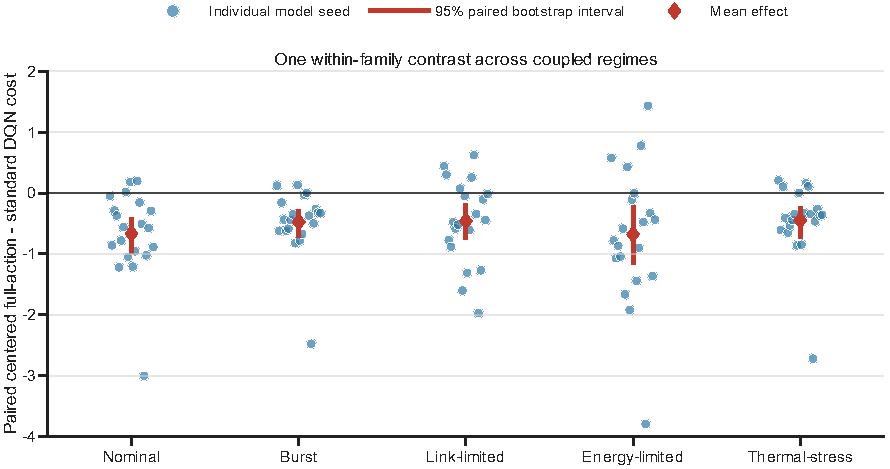
\includegraphics[width=0.98\textwidth]{figures/fig_seed_effects.pdf}
\caption{Paired total-cost differences for all 20 independent model seeds. Blue points show individual seed-level effects after averaging 20 shared traces. Red diamonds and vertical lines show mean differences and paired 95\% bootstrap intervals.}
\label{fig:seed_effects}
\end{figure}

\begin{table}[H]
\centering
\color{red}% BEGIN STATE-COMPLETE REVISION
\caption{Sensitivity of the centered full-action--standard DQN comparison to ignoring the prespecified model-seed matching. The two groups of 20 seed means are resampled independently. These intervals quantify the loss of precision when the common-random-number blocks are discarded and are not the primary analysis.}
\color{black}% END STATE-COMPLETE REVISION
\label{tab:unpaired}
\resizebox{0.80\textwidth}{!}{\begin{tabular}{lrrr}
\toprule
Regime & Mean difference & Unpaired 95\% interval & Excludes zero \\
\midrule
Nominal & -0.67 & [-1.79, 0.46] & No \\
Burst & -0.48 & [-1.66, 0.73] & No \\
Link-limited & -0.46 & [-1.56, 0.60] & No \\
Energy-limited & -0.68 & [-1.80, 0.48] & No \\
Thermal-stress & -0.45 & [-1.62, 0.77] & No \\
\bottomrule
\end{tabular}}
\end{table}

\color{red}% BEGIN STATE-COMPLETE REVISION
The primary result appears at the DQN-family level. In every fully coupled regime, the highest mean among the six DQN objectives remained below every implemented non-DQN mean. MPC-4 was the strongest non-DQN comparator in each regime. Consequently, all \DQNFamilyBelowMPCCount{} DQN objective--regime means were below their corresponding MPC-4 mean. Nominal DQN-family means ranged from \DQNFamilyNominalMinCost{} to \DQNFamilyNominalMaxCost, compared with \MPCNominalCost{} for MPC-4 and 101.00 for the contextual bandit. Fixed-onboard and fixed-ground means were 208.94 and 299.56, respectively. This ordering persisted across target designs and four resource-stress regimes, making family-level consistency the central benchmark result. Between-family inference remains descriptive because learned and deterministic methods express different sources of variation.
\color{black}% END STATE-COMPLETE REVISION

\color{red}% BEGIN STATE-COMPLETE REVISION
Differences within the DQN family were substantially smaller. Centered full-action supervision reduced standard-DQN mean cost by \PhysicalCBADMinPct--\PhysicalCBADMaxPct{} across the five coupled regimes, and every paired 95\% interval lay below zero. It was lower for \PrimaryNegativeSeedsMin--\PrimaryNegativeSeedsMax{} of 20 seed blocks, and every leave-one-seed-out mean remained negative (Table~\ref{tab:primary_inference}). The complete prespecified rule supported \PrimarySupportedCount{} regimes, while link-limited and thermal-stress retained favorable directional effects. The independent-seed bootstrap was wider and excluded zero in a subset of regimes (Table~\ref{tab:unpaired}). These results prioritize the family-level conclusion while allowing objective selection to remain scenario specific.
\color{black}% END STATE-COMPLETE REVISION

\color{red}% BEGIN STATE-COMPLETE REVISION
At $c=0$, immediate argmin and MPC-4 were identical; at $c=0.5$, MPC-4 had the lowest mean. The DQN-family advantage therefore emerged under the fully coupled conditions that match training. These boundary rows jointly change transition carryover and penalty scale, and they transfer $c=1$ policies without retraining. Orthogonal coupling controls and regime-specific retraining are natural extensions. MPC-4 required \MPCNominalPlanningMs{} ms per decision on the evaluation workstation.

\subsection{Target design fine-tunes performance within a consistently strong DQN family}
\color{black}% END STATE-COMPLETE REVISION

\begin{table}[H]
\centering
\color{red}% BEGIN STATE-COMPLETE REVISION
\caption{Episode total cost across six DQN-family objectives in the five fully coupled regimes. Values are mean $\pm$ SD across 20 independently trained model-seed blocks after within-seed averaging of 20 shared held-out traces. Lower is better; no row is designated as a uniformly preferred method.}
\label{tab:dqn_family}
\resizebox{\textwidth}{!}{\input{generated/table_dqn_family_performance.tex}}
\end{table}

\begin{figure}[H]
\centering
\includegraphics[width=0.98\textwidth]{figures/fig_dqn_family.pdf}
\caption{DQN-family performance across fully coupled regimes. Points show model-seed means and error bars show $\pm$1 SD across 20 independently trained model seeds. The figure emphasizes overlap and scenario-dependent ordering rather than a single winning objective.}
\label{fig:dqn_family}
\end{figure}

\begin{table}[H]
\centering
\caption{Nominal fixed-coefficient component and backbone comparisons. All models use 20 prespecified model-seed blocks, identical real-interaction budgets, and the same held-out traces. Full-action Q and immediate advantage receive the same three modeled action outcomes as the centered full-action variant. The shared $\lambda=0.3$ was calibrated for the centered objective and not tuned separately for the other auxiliary losses, so these rows do not isolate centering or bootstrapping. Holm adjustment covers the five fully coupled regimes separately for each displayed contrast. ``Supported'' requires a favorable mean, a paired interval below zero, and Holm $p<0.05$.}
\color{black}% END STATE-COMPLETE REVISION
\label{tab:extended_ablation}
\resizebox{\textwidth}{!}{\input{generated/table_extended_ablation.tex}}
\end{table}

\color{red}% BEGIN STATE-COMPLETE REVISION
\begin{table}[H]
\centering
\caption{Training information and computation accounting. Wall time is mean $\pm$ SD across 20 models. ``Modeled action outcomes'' counts analytical action evaluations used by the learning objective. Equal real interactions therefore do not imply equal information or computational budgets.}
\label{tab:training_accounting}
\resizebox{0.92\textwidth}{!}{\input{generated/table_training_accounting.tex}}
\end{table}
\color{black}% END STATE-COMPLETE REVISION

\color{red}% BEGIN STATE-COMPLETE REVISION
Table~\ref{tab:dqn_family} and Fig.~\ref{fig:dqn_family} show substantial overlap among the six DQN objectives. Nominal means span only \DQNFamilyNominalMinCost--\DQNFamilyNominalMaxCost, compared with the larger separation from MPC-4 and the contextual bandit. Target construction therefore fine-tunes performance within a DQN family whose shared advantage is more pronounced than its internal ordering.

The direct contrasts clarify this internal ordering. Full-action Q differed from standard DQN by \FullQDifference{} in nominal conditions and satisfied the complete rule in \FullQSupportedCount{} regimes. Centering changed full-action performance by \CenteredDifference{} [\CenteredCILow,\CenteredCIHigh], with Holm-adjusted $p=\CenteredHolmP$, and was supported in \CenteredSupportedCount{} regimes. Immediate-advantage supervision differed from standard DQN by \ImmediateDifference. The centered full-action-minus-immediate contrast was \BootstrapDifference{} [\BootstrapCILow,\BootstrapCIHigh], with Holm-adjusted $p=\BootstrapHolmP$. The Double-DQN contrast was \DoubleDifference{} [\DoubleCILow,\DoubleCIHigh], with Holm-adjusted $p=\DoubleHolmP$, and was supported in \DoubleSupportedCount{} regimes. Centered full-action objectives repeatedly achieved favorable means, but the shared DQN formulation accounted for the larger performance separation.

\subsection{Deeper exact planning improves cost but retains a gap to the DQN family}
\color{black}% END STATE-COMPLETE REVISION

\begin{table}[H]
\centering
\color{red}% BEGIN STATE-COMPLETE REVISION
\caption{Nominal receding-horizon planning over 400 unique held-out traces. Each planner has perfect knowledge of the next $H$ tasks and exogenous link states and exactly enumerates $3^H$ sequences before every action. Runtime was measured on the same workstation and includes only planner action selection after environment construction. DQN inference time was not benchmarked in this experiment, so the table is not a matched deployment-latency comparison.}
\color{black}% END STATE-COMPLETE REVISION
\label{tab:planner_depth}
\resizebox{0.85\textwidth}{!}{\input{generated/table_planner_depth.tex}}
\end{table}

\color{red}% BEGIN STATE-COMPLETE REVISION
Increasing planning depth reduced nominal mean cost from \PlannerCostHOne{} at $H=1$ to \PlannerCostHTwo, \PlannerCostHFour, and \PlannerCostHSix{} at $H=2$, 4, and 6, respectively. Mean decision time increased from \PlannerTimeHOne{} to \PlannerTimeHSix{} ms across the same range. Even MPC-6 remained above the nominal DQN-family range of \DQNFamilyNominalMinCost--\DQNFamilyNominalMaxCost. Thus, the family-level ordering persisted as exact enumeration deepened within the tested horizon, while computational growth motivated scalable planning comparisons as a future extension.
\color{black}% END STATE-COMPLETE REVISION

\begin{table}[H]
\centering
\color{red}% BEGIN STATE-COMPLETE REVISION
\caption{Engineering outcome decomposition for centered full-action relative to standard DQN. Delta columns report centered full-action minus standard DQN. Negative values denote lower use or cost. Low-energy steps count decisions with remaining energy below 0.18; they are soft-threshold exposures, not certified safety violations.}
\color{black}% END STATE-COMPLETE REVISION
\label{tab:engineering}
\small
\setlength{\tabcolsep}{4pt}
\input{generated/table_engineering_outcomes.tex}
\end{table}

\color{red}% BEGIN STATE-COMPLETE REVISION
Table~\ref{tab:engineering} separates the composite objective into its modeled consequences. Across the displayed regimes, the centered full-action DQN objective reduced immediate cost and delayed penalty. It used slightly less modeled energy and latency while transmitting more data, revealing an allocation trade-off rather than uniform resource reduction. The low-energy count records exposure to the simulator's soft threshold. Both learned policies reached zero remaining energy, identifying hard-feasibility enforcement as an important next step. Under thermal stress, the policies accommodated elevated initial heat and contiguous load without crossing the modeled heat threshold.
\color{black}% END STATE-COMPLETE REVISION

\color{red}% BEGIN STATE-COMPLETE REVISION
\subsection{Representative DQN training diagnostics show empirical stabilization}
\color{black}% END STATE-COMPLETE REVISION

\begin{figure}[H]
\centering
\includegraphics[width=0.98\textwidth]{figures/fig_training_diagnostics.pdf}
\color{red}% BEGIN STATE-COMPLETE REVISION
\caption{Representative training diagnostics for standard DQN and the centered full-action DQN variant. Lines are means across 20 model seeds after a causal 25-episode moving average; shaded regions are $\pm$1 SD. Curves describe the training distribution and are not used as independent test observations or evidence for the whole DQN family.}
\color{black}% END STATE-COMPLETE REVISION
\label{fig:training}
\end{figure}

\color{red}% BEGIN STATE-COMPLETE REVISION
All four logged quantities declined rapidly during the first approximately 220 episodes and then fluctuated around a stable range (Fig.~\ref{fig:training}). Across seeds and episodes 501--600, the centered full-action variant averaged \LateCBADCost{} total cost, \LateCBADEnergy{} normalized energy use, \LateCBADLatency{} s latency, and \LateCBADPenalty{} delayed penalty. Standard DQN averaged \LateDQNCost, \LateDQNEnergy, \LateDQNLatency{} s, and \LateDQNPenalty, respectively. These curves answer the optimization question without reintroducing the undefined ``accuracy'' metric. They show empirical stabilization, not mathematical convergence.
\color{black}% END STATE-COMPLETE REVISION

\color{red}% BEGIN STATE-COMPLETE REVISION
\subsection{Within-family sensitivity under parameter changes}
\color{black}% END STATE-COMPLETE REVISION

\begin{table}[H]
\centering
\color{red}% BEGIN STATE-COMPLETE REVISION
\caption{Prespecified parameter sensitivity for centered full-action minus standard DQN. Negative differences favor the centered full-action variant; $n=20$ independent paired model seeds in each profile. Holm adjustment covers the eight displayed profiles.}
\color{black}% END STATE-COMPLETE REVISION
\label{tab:sensitivity}
\resizebox{0.84\textwidth}{!}{\input{generated/table_sensitivity.tex}}
\end{table}

\begin{figure}[H]
\centering
\includegraphics[width=0.98\textwidth]{figures/fig_sensitivity_planning.pdf}
\color{red}% BEGIN STATE-COMPLETE REVISION
\caption{Parameter sensitivity and planning boundary. (a) Mean paired centered full-action--standard DQN differences with 95\% paired bootstrap intervals. (b) Immediate, four-step rolling, and learned scheduling across coupling and stress regimes.}
\color{black}% END STATE-COMPLETE REVISION
\label{fig:sensitivity}
\end{figure}

\color{red}% BEGIN STATE-COMPLETE REVISION
The paired centered-full-action--standard-DQN interval remained below zero in all eight profiles, with relative differences from \SensitivityMinPct{} to \SensitivityMaxPct. The largest tested difference occurred when raw data volume decreased by 20\%, whereas the smallest occurred when it increased by 20\%. This directional stability supports the within-family pattern across the prespecified parameter envelope and motivates evaluation under broader mission-derived distributions.
\color{black}% END STATE-COMPLETE REVISION

\color{red}% BEGIN STATE-COMPLETE REVISION
\subsection{Preview-scale perturbations bound one model-assisted variant}
\color{black}% END STATE-COMPLETE REVISION

\begin{table}[H]
\centering
\color{red}% BEGIN STATE-COMPLETE REVISION
\caption{Effect of training-time preview misspecification. Differences are relative to the same standard-DQN models evaluated in the factual simulator. Scaling applies only to the centered full-action variant's training-time preview cost and action-induced resource changes.}
\color{black}% END STATE-COMPLETE REVISION
\label{tab:preview_mismatch}
\resizebox{\textwidth}{!}{\input{generated/table_preview_mismatch.tex}}
\end{table}

\color{red}% BEGIN STATE-COMPLETE REVISION
Table~\ref{tab:preview_mismatch} tests uniform 15\% under- and over-scaling of modeled one-step consequences. The 0.85 and 1.15 conditions satisfied the complete rule in \MismatchLowSupportedCount{} and \MismatchHighSupportedCount{} regimes, respectively. Their largest Holm-adjusted sign-test values were \MismatchLowHolmPMax{} and \MismatchHighHolmPMax. Remaining rows provide directional sensitivity evidence. The tested scale perturbations preserve the favorable pattern and motivate future evaluation of structural, state-dependent, and action-specific preview errors.
\color{black}% END STATE-COMPLETE REVISION

\color{red}% BEGIN STATE-COMPLETE REVISION
\subsection{A centered full-action policy uses different action mixtures across regimes}
\color{black}% END STATE-COMPLETE REVISION

\color{red}% BEGIN STATE-COMPLETE REVISION
The centered full-action policy did not collapse to one processing mode. Its mean action fractions changed across regimes, including greater onboard execution under link limitation. Figure~\ref{fig:actions} therefore provides descriptive evidence of regime-dependent allocation, while family-wide action-mechanism analysis remains a future direction.
\color{black}% END STATE-COMPLETE REVISION

\begin{figure}[H]
\centering
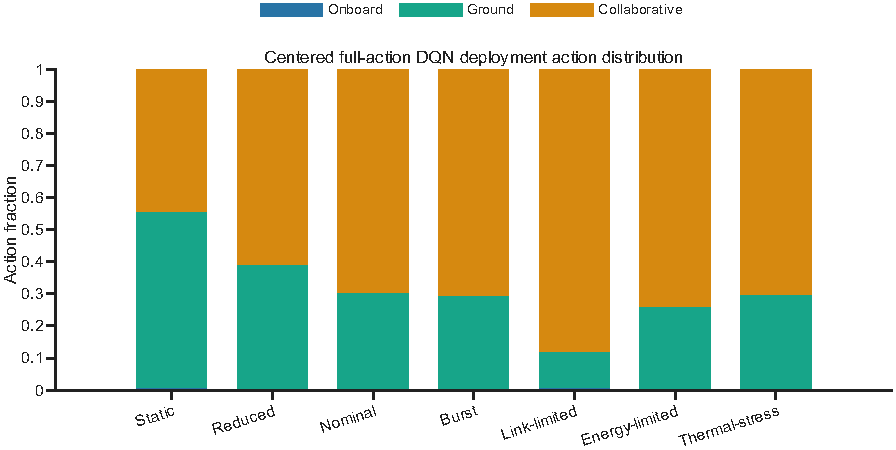
\includegraphics[width=0.90\textwidth]{figures/fig_reviewer_actions.pdf}
\color{red}% BEGIN STATE-COMPLETE REVISION
\caption{Mean deployment action fractions for the centered full-action DQN variant under the internally consistent synthetic generator. Values are descriptive means across evaluated traces; no uncertainty or within-family comparison is shown.}
\color{black}% END STATE-COMPLETE REVISION
\label{fig:actions}
\end{figure}

\color{red}% BEGIN STATE-COMPLETE REVISION
\section{Discussion}
\color{black}% END STATE-COMPLETE REVISION

\color{red}% BEGIN STATE-COMPLETE REVISION
The central finding is the consistency of the DQN family across objective designs and operating regimes. In all five fully coupled regimes, every DQN objective achieved a lower mean cost than every implemented non-DQN comparator. This ordering survived changes in model supervision, centering, bootstrapping, and Double-DQN evaluation. The contextual bandit's higher costs further show that immediate-reward learning did not reproduce the advantage of long-horizon DQN targets. The shared family-level pattern is therefore more consequential than the smaller differences among individual objectives.
\color{black}% END STATE-COMPLETE REVISION

\color{red}% BEGIN STATE-COMPLETE REVISION
Within-family comparisons refine this conclusion. Centered full-action supervision produced favorable paired means across all five coupled regimes, although the complete rule supported \PrimarySupportedCount{} regimes. Full-action Q, immediate advantage, and Double-DQN controls showed that several target constructions can occupy a narrow performance band. Convergence across these objectives makes the main result less dependent on one named formulation. It also indicates that target design should be selected for the operating regime rather than treated as universally ranked.
\color{black}% END STATE-COMPLETE REVISION

\color{red}% BEGIN STATE-COMPLETE REVISION
The planning analysis provides a second perspective on the result. MPC-6 reduced nominal mean cost to \PlannerCostHSix{} using perfect knowledge of the next six tasks. Its cost nevertheless remained above the complete nominal DQN-family range of \DQNFamilyNominalMinCost--\DQNFamilyNominalMaxCost. Meanwhile, exact-enumeration time increased from \PlannerTimeHOne{} to \PlannerTimeHSix{} ms per decision between $H=1$ and $H=6$. The comparison therefore identifies a clear quality--computation frontier for transparent finite-horizon planning in the benchmark.
\color{black}% END STATE-COMPLETE REVISION

\color{red}% BEGIN STATE-COMPLETE REVISION
The benchmark itself provides an additional methodological contribution. Heat, energy, latency, and transmitted volume are derived from shared task primitives rather than sampled independently. Complete transition equations, fixed-seed audits, and generated result tables connect each reported value to executable artifacts. This design makes the family-level comparison reproducible and exposes which assumptions must change when the benchmark is transferred to another mission setting.
\color{black}% END STATE-COMPLETE REVISION

\color{red}% BEGIN STATE-COMPLETE REVISION
\subsection{Future work}

The first priority is to move from soft feasibility accounting to operational constraint enforcement. Action masking, constrained reinforcement learning, and terminal resource conditions can prevent infeasible energy trajectories. Mission-derived utility weights, telemetry, and hardware-in-the-loop traces can then test whether the observed ordering persists under physical resource dynamics. Extending the topology to multiple satellites, ground stations, and contact opportunities would further test scalability.

The second priority is sharper mechanism identification. Future experiments should tune auxiliary weights by objective, normalize gradient contributions, and factorially separate centering from Bellman bootstrapping. Transition carryover and delayed-penalty scaling should also be varied independently instead of sharing the coupling coefficient $c$. Broader discount factors, utility weights, and structural preview errors would reveal which components sustain the within-family patterns.

The third priority is a wider algorithmic frontier. Scalable tree search, dynamic programming, mixed-integer optimization, and satellite-specific schedulers should be compared under matched information and computation budgets. Modern value-learning components and additional sequential tasks can test whether the family-level finding transfers beyond the current architecture. Matched inference-latency and energy measurements would complete the deployment comparison. Together, these steps can convert a controlled benchmark result into operationally transferable evidence.
\color{black}% END STATE-COMPLETE REVISION

\section{Conclusion}

\color{red}% BEGIN STATE-COMPLETE REVISION
We present a reproducible resource-coupled benchmark and a controlled comparison of six DQN objectives. Across five fully coupled regimes, all \DQNFamilyBelowMPCCount{} DQN objective--regime means were below the strongest implemented non-DQN comparator, MPC-4. In nominal conditions, even MPC-6 remained above the complete DQN-family range despite perfect six-task foresight. Differences among DQN objectives were smaller and scenario dependent, making family-level consistency the principal contribution. The results show that long-horizon DQN value learning can provide a strong scheduling strategy within this benchmark. Future mission-calibrated, hard-constrained, and multi-satellite studies will determine how broadly this advantage transfers.
\color{black}% END STATE-COMPLETE REVISION

\section*{Funding}

This work was supported by the National Key Research and Development Program of China under Grants 2022YFF0503904 and 2022YFD2401202. Additional support came from the Shenzhen Higher Education Institutions Stabilization Support Program under Grant GXWD\allowbreak20220811163556003. The National Natural Science Foundation of China supported this work under Grant 62202127, and the Shenzhen Natural Science Foundation under Grant JCYJ\allowbreak20241202123731040. Further support came from the Guangxi Science and Technology Base and Talent Special Project under Grant Gui Ke AD25069103.

\section*{Data and Code Availability}

\color{red}% BEGIN STATE-COMPLETE REVISION
The local versioned research package contains the simulator, checkpoints, raw evaluations, seed-level summaries, fixed-seed inference, direct Python dependencies, MATLAB figure source, and LaTeX-table generators under \texttt{md\_cbad\_dqn/}. It includes the primary, preview-error, component-control, and Double-DQN results. Machine-readable validation and metadata files record expected rows, model seeds, training budgets, randomization blocks, package versions, and result hashes. The commands in the reproducibility subsection regenerate the result chain. A permanent public archive has not yet been supplied for review. \textbf{AUTHOR ARCHIVE IDENTIFIER TO BE INSERTED BEFORE SUBMISSION.}
\color{black}% END STATE-COMPLETE REVISION

\begingroup
\small
\setlength{\itemsep}{0.2em}
\bibliographystyle{unsrt}
\bibliography{ref}
\endgroup

\end{document}
